\section{Introduction}
In this paper, we will look at the behavior of curves on the projective plane. Although we will focus on results in algebraically closed fields the following results only require that the intersection points exist in the projective plane.

\subsection{The Projective Plane and Curves}
We will start by giving algebraic definitions of affine and projective space. Throughout this paper, we will fix a field $k$ that is algebraically closed.
\begin{definition}
For a field $k$ the $n$ dimensional projective space is 
$$\P^n=\{[x_1:x_2:\dots:x_{n+1}]|x_1,x_2,\dots,x_{n+1}\text{ not all zero}\}/\sim$$
Which is isomorphic to the space $k^{n+1}-0$ modded out by the relation that relates $[x_1:x_2:\dots:x_{n+1}]\sim [y_1:y_2:\dots:y_{n+1}]$ if and only if $x_i=ty_i$ for $t\in k-0$ for all $i$.
\end{definition}
%\begin{definition}
%    In $\P^n$ we may consider a subspace, denoted $\A^n$ to be the affine space of dimension $n$ if it is isomorphic to $k^n$, the $n$ dimensional vector space of $k$.
%\end{definition}
\begin{prop}
\label{prop:affine_def}
    The projective space $\P^n$ can be turned into the affine space $\A^n$ with the removal of any hyper plane in $\P^n$
\end{prop}
%\begin{proof}
%    Consider a line $F(x,y,z)=ax+by+cz=0$ And notice that the removal of such a line is equivalent to considering the points $[x:y:z]$ such that $F(x,y,z)\neq 0$, and WLOG we may scale the values of $x,y$ and $z$ and assume that $F(x,y,z)=1$. Furthermore $a,b$, and $c$ can not all be zero, and so WLOG assume that $c$ is non zero. This means for any choice of $x$ and $y$ we have that the point $[x:y:\frac{1-ax-by}{c}]$. This defines the map $k^2\hookrightarrow \P^2$ such that $(x,y)\mapsto [x:y:\frac{1-ax-by}{c}]$ giving the affine space $\A^2$ to be the points not on the line $F(x,y,z)=0$. Furthermore notice that $(x+y)+\ell(u,v)\mapsto [x:y:\frac{1-ax-by}{c}]+[\ell u:\ell v:\frac{1-a\ell u-b\ell v}{c}]=[x+\ell u:y+\ell v:\frac{1-a(x+\ell u)-b(y+\ell v)}{c}]=:P$ such that $F(P)=a(x+\ell u)+b(y+\ell v)+1-a(x+\ell u)-b(y+\ell v)=$ This defined a linear transformation with the points in $\P^2$
%\end{proof}

\begin{example}
    When $n=2$ we call $\P^2=\{[x:y:z]|x,y,z\text{ not all zero}\}/\sim$ the projective plane. Notice that in this case we may remove the line $z=0$ which means $z\neq 0$ and so up to scaling we may fix $z=1$, which are the points of the form $[x:y:1]$ which can be interpreted as the affine space $k^2$, with the bijection mapping $(x,y)\mapsto [x:y:1]$. 
\end{example}
 Notice that because projective transformations take lines to lines we may assume any affine space can be interpreted as $\A^2=\{[x:y:z]\in \P^2|z=1\}\cong k^2$ up to linear transformation. 
  
  Therefore the line that is removed to create $\A^2$, which we may assume to be $z=0$ can be interpreted as the line at infinity, and behaves as a closure of $\A^2\cong k^2$.

For example consider values $a, b\in k$ and consider the limit of a sequence of points in $k^2$ that is $\lim_{t\ra\infty}(ta,tb)$. In projective space we may interpret this limit as $\lim_{t\ra\infty}[ta:tb:1]$ and with rescaling by $t$ we may notice that $\lim_{t\ra\infty}[ta:tb:1]=\lim_{t\ra\infty}[a:b:1/t]=[a:b:0]$ which is a point at infinity, encoding the direction in which the sequence approached infinity.

Now we will create definitions for curves in affine space which we can extend to curves in projective space. 

\begin{definition}
    A curve $C$ in the affine plane $\A^2$ is the set of solutions to a polynomial equation $f(x,y)=0$ where $f\in k[x,y]$. We may denote such a curve as $C:f(x,y)=0$.
\end{definition}
As in the definition of projective space, projective curves must be invariant under the scaling of the entries. 
\begin{definition}
    A projective curve $C$ of degree $d$ in $\P^2$ is the set of solutions to a non-constant polynomial equation $F(x,y,z)=0$ where $F$ is a \textit{homogeneous polynomial} of degree $d$, that is $F\in k[x,y,z]$ is the sum of degree $d$ monomials such that $F(tx,ty,tz)=t^dF(x,y,z)$.
\end{definition}
%Notice that this definition requires that every term in the polynomial $F$ has degree $d$, meaning projective curves are linear combinations of degree $d$ monomials.
Notice first that for every projective curve $C:F(x,y,z)$ we can extract an affine curve by removing a hyperplane, for example removing $z=0$ and scaling $z=1$. That is the affine part of $F$ is the curve $f(x,y)=F(x,y,1)$ where any projective point in affine space, $[a:b:1]$ we have that $F(a,b,1)=0$ if and only if $f(a,b)=0$. This process is called dehomogenization. Not all projective curves have affine components, for example, the curve $z=0$ is only defined at infinity and has no non-constant dehomogenized polynomial in $k[x,y]$. However with the removal of another line ($x=0$ for example), and therefore another perspective of $\A^2$, this curve would have an affine part. 

Points at infinity, when $z=0$, correspond to the slopes of the curve or how the curve approaches infinity, this can be formalized in a similar way as in the previous limit example.

Similar to the process of dehomogenization which extracts affine components of projective curves we can create a process of homogenization that takes an affine curve of degree $d$ to a projective curve of degree $d$ with a correspondence of its affine points. That is given an affine curve of degree $d$ defined by the polynomial $f(x,y)=\sum_{i,j}a_{ij}x^iy^j$ we define the degree $d$ homogenization as the polynomial $F(x,y,z)=\sum_{i,j}a_{ij}x^iy^jz^{d-i-j}$. Notice that $f(x,y)=F(x,y,1)$, and so both curves share affine points. Furthermore, by construction $F(x,y,0)$ is not identically zero for all $x$ and $y$, meaning $z$ is not a common factor and so $F$ does not contain the line at infinity $z=0$. The processes of homogenization and dehomogenization define a bijection between affine curves and projective curves that do not contain the line at infinity $z=0$.

\subsection{Intersecting Curves}
In studying curves there is often the question of the number of intersecting points.
\begin{definition}
    Given two curves $C_1:F(x,y,z)=0$ and $C_2:G(x,y,z)=0$ we say that a point $[a:b:c]$ is in the intersection $C_1\cap C_2$ if $[a:b:c]$ is simultaneously a point of $C_1$ and $C_2$, that is $F(a,b,c)=G(a,b,c)=0$.
\end{definition}
A similar definition can be made for affine curves. In general, we are only interested in the case where the number of intersection points is finite, the case that two curves share no common components.
\begin{definition}
    If $k[x,y]$ is a UFD then we may factor a projective curve as $F(x,y,z)=p_1(x,y,z)p_2(x,y,z)\cdots p_r(x,y,z)$ into the product of irreducible polynomial factors $p_i(x,y,y)\in k[x,y]$. We say that the \textit{irreducible components} of $C$ are the polynomials $p_i(x,y,z)$ for all $i$. We say two curves have no common components if their irreducible factors are distinct.
\end{definition}
In our case where $k$ is a field, $k[x,y]$ is always a UFD.

It is often the case that intersections will include multiplicity, for example, these are the cases where two curves share tangent lines. We may interpret the multiplicity to be the number of derivatives the curves share. Formally we define this notion with local rings.

\begin{definition}
\label{def:localring_P}
    Let $k$ be algebraically closed, then let $K\leq k(x,y,z)$ with elements that are rational functions of the form $\Phi=F/G$, with $F, G$ being homogeneous polynomials of $x,y$ and $z$ of the same degree. For a point $P\in\P^2$, we say that $\Phi$ is defined at $P$ if $G(P)\neq 0$. And the local ring of a point $P$ is the space $\mathcal{O}_P=\{\Phi\in K| \Phi \text{ is defined at }P\}$.
\end{definition}

Notice that for projective curves defined by polynomials $F_1,F_2$ an ideal of $\mathcal{O}_P$ is defined as 
\begin{equation}
\label{eq:ideal_pspace}
    \ip{F_1,F_2}_P=\{F/G\in\mathcal{O}_P| F=H_1F_1+H_2F_2 \}
\end{equation}
Where $H_1,H_2\in k[X,Y,Z]$ such that $F$ is homogeneous of degree equal to that of $G$.
We can also restrict these constructions to the affine plane.

\begin{prop}
\label{prop:localring_A}
If $P=(a,b)=[a:b:1]\in A$ then we may instead define $K\leq k(x,y)$ with elements that are rational functions of the form $\phi=f/g$, with $f,g$ being polynomials of $x$ and $y$. For a point $P\in\A^2$, we say that $\phi$ is defined at $P$ if $g(P)\neq 0$. And the local ring of a point $P$ is the space $\mathcal{O}_P=\{\phi\in K| \phi \text{ is defined at }P\}$.
\end{prop}
\begin{proof}
These definitions coincide with definition \ref{def:localring_P} through the process of dehomoginization.
\end{proof}

Likewise for affine curves defined by polynomials $f_1,f_2$ an ideal of $\mathcal{O}_P$ is defined as $\ip{f_1,f_2}_P=\mathcal{O}_Pf_1+\mathcal{O}_Pf_2$ which agree with equation \ref{eq:ideal_pspace}.

This then allows us to define the multiplicity of the intersection of two curves
\begin{definition}
\label{def:intmult}
    For curves $C_1:F_1(x,y,z)=0$ and $C_2:F_2(x,y,z)=0$ and a point $P\in\P^2$ we have that 
    $$I(C_1\cap C_2,P)=\dim(\mathcal{O}_P/\ip{F_1,F_2}_P)$$
    And if $P\in \A^2$ we have the alternative definition $I(C_1\cap C_2,P)=\dim(\mathcal{O}_P/\ip{f_1,f_2}_P)$ where $f_1,f_2$ represent the affine parts of $F_1$ and $F_2$.
\end{definition}
Below we have given a few examples using this definition
\begin{example}
\label{ex:int1}
Consider the projective curves $C_1:F_1(x,y,z)=x+z=0$ and $C_2:F_2(x,y,z)=x^2-yz=0$, where $C_1$ is a line and $C_2$ is a quadratic. The restriction of both curves in the affine plane (from the removal of $z=0$ and then scaling $z=1$), where $f_1(x,y)=x+1$ and $f_2(x,y)=x^2-y$ is shown in figure \ref{fig:int1}. $C_1$ and $C_2$ intersect at the affine point $[-1:1:1]$ and the projective point $[0:1:0]$ encoding that the curves go off to infinity vertically. We will show that for the affine point $P=(-1,1)$, that $I(C_1\cap C_2,P)=1$. To show this it suffices to show that $\ip{f_1,f_2}_P=\mathcal{M}_P:=\{\phi\in \mathcal{O}_P| \phi(P)=0\}$, which can be done by showing $\ip{f_1,f_2}_P$ contains all degree $1$ polynomials that go through $(-1,1)$. To see this notice that $(x-1)(x+1)=x^2-1$ and so $(x^2-1)-(x^2-y)=y-1$. This means that $x+1,y-1\in\ip{f_1,f_2}_P$ which generates all polynomials that go through $(-1,1)$.
\begin{figure}
    \centering
    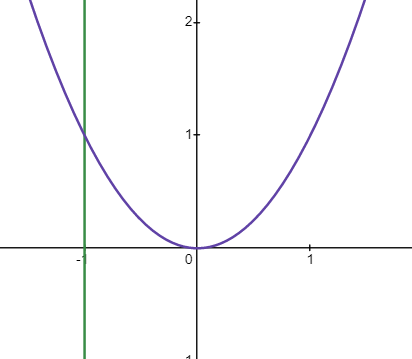
\includegraphics[scale=.5]{pics/graph2.png}
    \caption{The intersection of $C_1:x+1=0$ shown in green and $C_2:x^2-y=0$ in purple from example \ref{ex:int1}.}
    \label{fig:int1}
\end{figure}
\end{example}
\begin{example}
\label{ex:int2}
Now we will show an example with an intersection of higher multiplicity to motivate an interpretation of multiplicity. Consider the projective curves $C_1:F_1(x,y,z)=x-y+2z=0$ and  $C_2:F_2(x,y,z)=x^2+xz-yz+2z^2=0$, where $C_1$ is a line and $C_2$ is a quadratic. The restriction of both curves in the affine plane (from the removal of $z=0$ and then scaling $z=1$), where $f_1(x,y)=x-y+2$ and $f_2(x,y)=x^2+x-y+2$ is shown in figure \ref{fig:int2}. $C_1$ and $C_2$ intersect at the affine point $[0:2:1]$. Notice that because $x^2+x-y+2-(x-y+2)=x^2$ we have that $\ip{f_1,f_2}_P=\ip{x-y+2,x^2}_P$. Notice that this means $\mathcal{O}_P/\ip{f_1,f_2}_P$ is spanned by the parallel classes of $1$ and $x$, and so has dimension $2$. To see this another way we may consider the Taylor expansions of both curves with respect to $y$, that is $y=2+1\cdot x$ and $y=2+1\cdot x+1\cdot x^2$, where we see that both curves share a derivatives at the point of intersection. This motivates that the intersection multiplicity counts the number of shared derivatives. However this interpretation does not extend to all fields, such as finite fields.
\begin{figure}
    \centering
    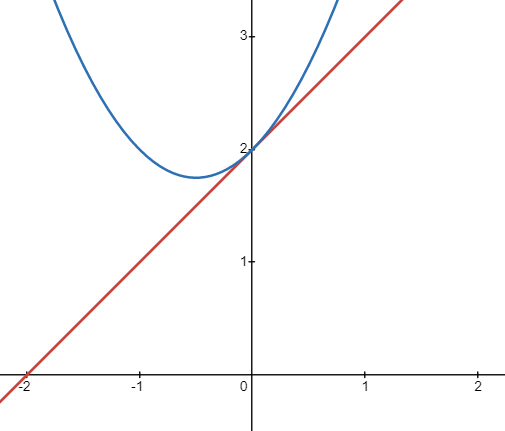
\includegraphics[scale=.5]{pics/graph1.png}
    \caption{The intersection of $C_1:x-y+2=0$ shown in red and $C_2:x^2+x-y+2=0$ in blue from example \ref{ex:int2}.}
    \label{fig:int2}
\end{figure}
\end{example}

\begin{example}
\label{ex:int3}
    Now we will show an example with an intersection of multiplicity $3$. Consider the projective curves $C_1:F_1(x,y,z)=z^3+x^3-yz^2=0$ and  $C_2:F_2(x,y,z)=z-y=0$. The restriction of both curves in the affine plane (from the removal of $z=0$ and then scaling $z=1$), where $f_1(x,y)=1+x^3-y$ and $f_2(x,y)=1-y$ is shown in figure \ref{fig:int3}. $C_1$ and $C_2$ intersect at the affine point $[0:1:1]$. 
    Notice that because $1+x^3-y-(1-y)=x^3$ we have that $\ip{f_1,f_2}_P=\ip{1-y,x^3}_P$. Notice that this means $\mathcal{O}_P/\ip{f_1,f_2}_P$ is spanned by the parallel classes of $1$, $x$ and $x^2$, and so has dimension $3$. We may also see that both curves share a derivatives and a second derivative at the point of intersection. This again shows that the intersection multiplicity counts the number of shared derivatives.
    \begin{figure}
    \centering
    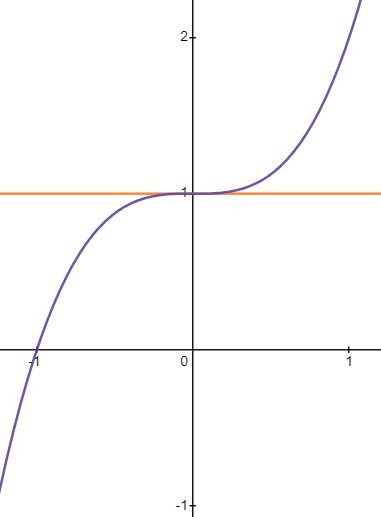
\includegraphics[scale=.5]{pics/graph3.png}
    \caption{The intersection of $C_1:1+x^3-y=0$ shown in purple and $C_2:1-y=0$ in orange from example \ref{ex:int3}.}
    \label{fig:int3}
\end{figure}
\end{example}

The following are expected facts about the intersection multiplicity
\begin{prop}
    $I(C_1\cap C_2,P)$ is a non-negative finite integer and $P\in C_1\cap C_2$ if and only if $I(C_1\cap C_2,P)\geq 1$
\end{prop}
\begin{proof}
    A proof of the first part of this statement is given in propositon \ref{prop:finitness_of_I}
\end{proof}

Now we will explore the intersection of curves with Bezout's Theorem
\begin{thm} (Bezout's theorem)
Let $C_1$ and $C_2$ be projective curves of degree $n_1$ and $n_2$ respectively with no common components then 
$$\sum_{P\in C_1\cap C_2} I(C_1\cap C_2, P)=n_1n_2$$
If every point in the intersection has an intersection of multiplicity $1$ then it is the case that $\#(C_1\cap C_2)=n_1n_2$. In all cases $\#(C_1\cap C_2)\leq n_1n_2$
\end{thm}

We will prove Bezout's theorem throughout the next section as outlined in \cite{silverman_rational_2015}.


